%%%%%%%%%%%%%%%%%%%%%%%%%%%%%%%%%%%%%%%%%%%%%%%%%%%%%%%%%%%%%%%%%%%%%%
%%                    Interaction
%%%%%%%%%%%%%%%%%%%%%%%%%%%%%%%%%%%%%%%%%%%%%%%%%%%%%%%%%%%%%%%%%%%%%%
\color{blue}

\subsection{Glyph: \glyph{Interaction}}\label{sec:interaction}

\glyph{Interaction} represents an interaction between two \glyph{entity} or \glyph{outcome}, whether non-covalent physical interaction, or functional interaction, e.g. genetic interaction. Each arrowhead points to an interactor involved in the interaction. The result of the interaction is represented by \glyph{outcomes} (see section \ref{sec:outcome}), that is by filled dots on the line linking the two arrowheads. The result of an interaction can be represented by any number of \glyph{outcomes}.

\begin{glyphDescription}
 \glyphSboTerm SBO:0000342 molecular or genetic interaction
 \glyphOrigin \glyph{entity} \sect{entity} or \glyph{outcome} \sect{outcome}.
 \glyphTarget \glyph{entity} \sect{entity} or \glyph{outcome} \sect{outcome}.
 \glyphEndPoint Both origin and target extremities of an \glyph{interaction} carry an harpoon arrowhead.
 \end{glyphDescription}

\begin{center}
\scalebox{0.5}{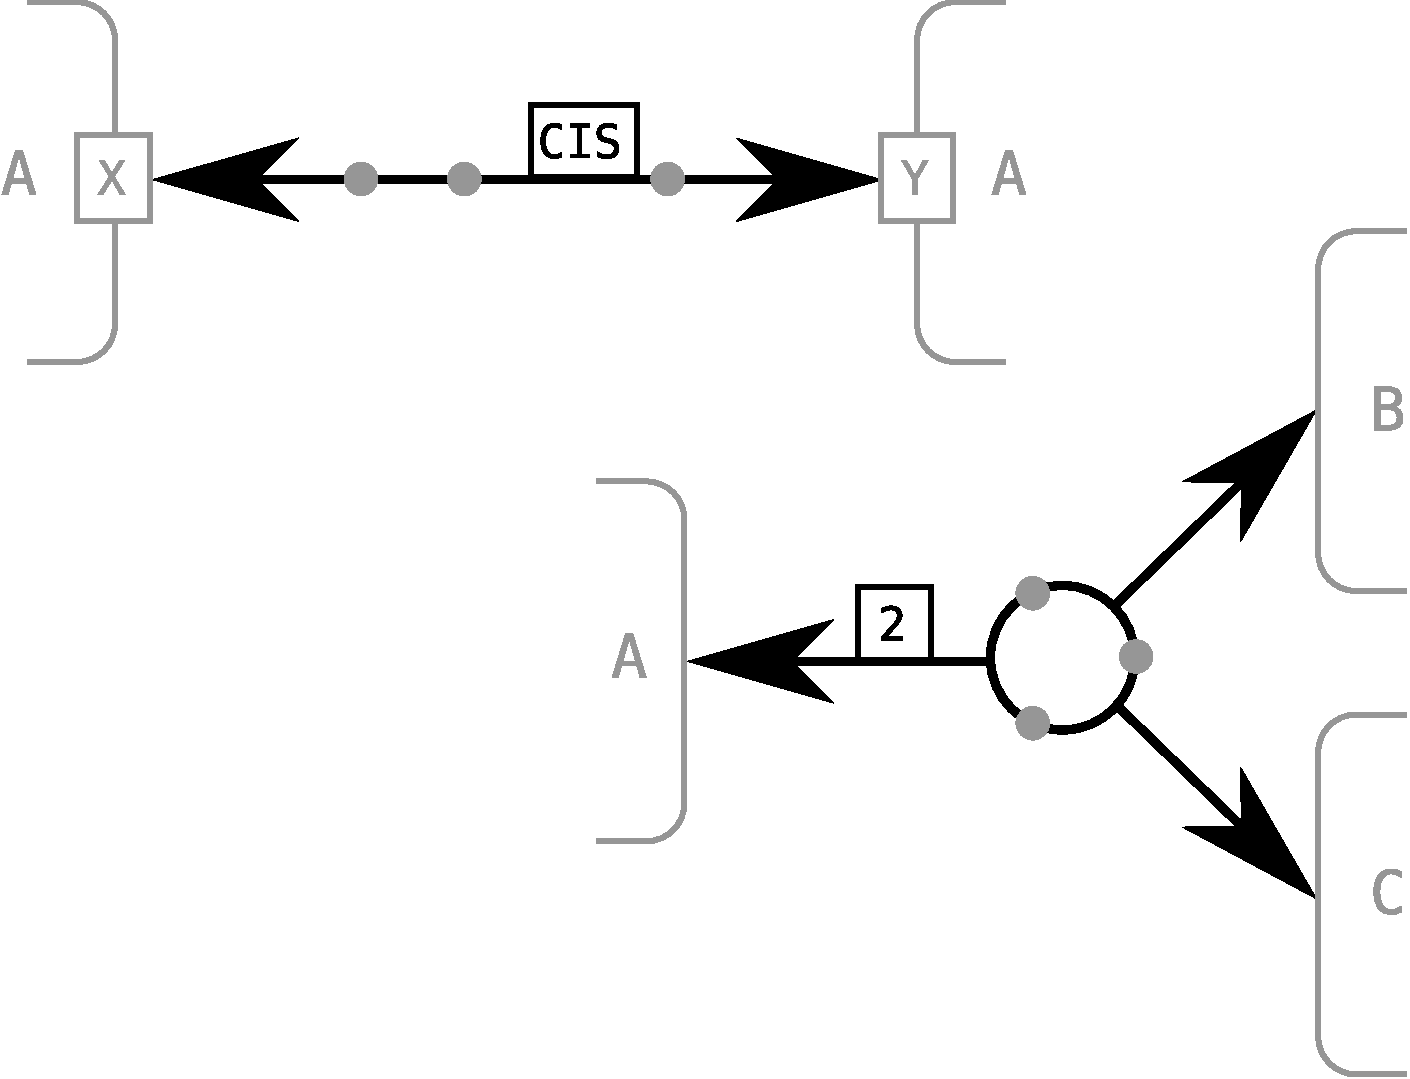
\includegraphics{images/interaction}}
\end{center}

\question{NLN}{TREAT THE CASE OF NON-BINARY INTERACTIONS}

 
% The following example illustrates the interaction of cyclin and CDC2 kinase to form the Maturation Promoting Factor in ER.
% 
% \begin{center}
% \scalebox{0.5}{\includegraphics{images/interaction-example1.eps}}
% \end{center}
\normalcolor

\newpage